\chapter{Teil 3: Engineering}
\label{chap:engineering}
\section{Webcrawler}
Dieser Abschnitt beschreibt sowohl die Technologie des Webcrawlers als auch die Erarbeitung dessen.
\subsection{Stand der Forschung}
Ein Webcrawler ist ein Programm, das automatisch das World Wide Web durchsucht und Webseiten analysiert\cite[p.311]{liu2007web}.
Ein Webcrawler braucht verwendet als Startpunkt ein Seed, welches URLs enthält.
Der Ablauf, welcher in \cref{fig:flowchart_webcrawler} gezeigt wird, ist wie folgt zu verstehen:
Die URLs aus dem Seed werden in eine Queue, genannt Frontier, geladen.
Von da aus werden diese Webpages aufgerufen und nach weiteren URLs durchsucht.
Die gefundenen URLs werden ebenfalls zum Frontier hinzugefügt, die Webpage selbst wird gespeichert.
Dieser Ablauf findet solange statt bis ein gewisses Ziel erreicht ist\cite[p.313]{liu2007web}.
\begin{figure}
	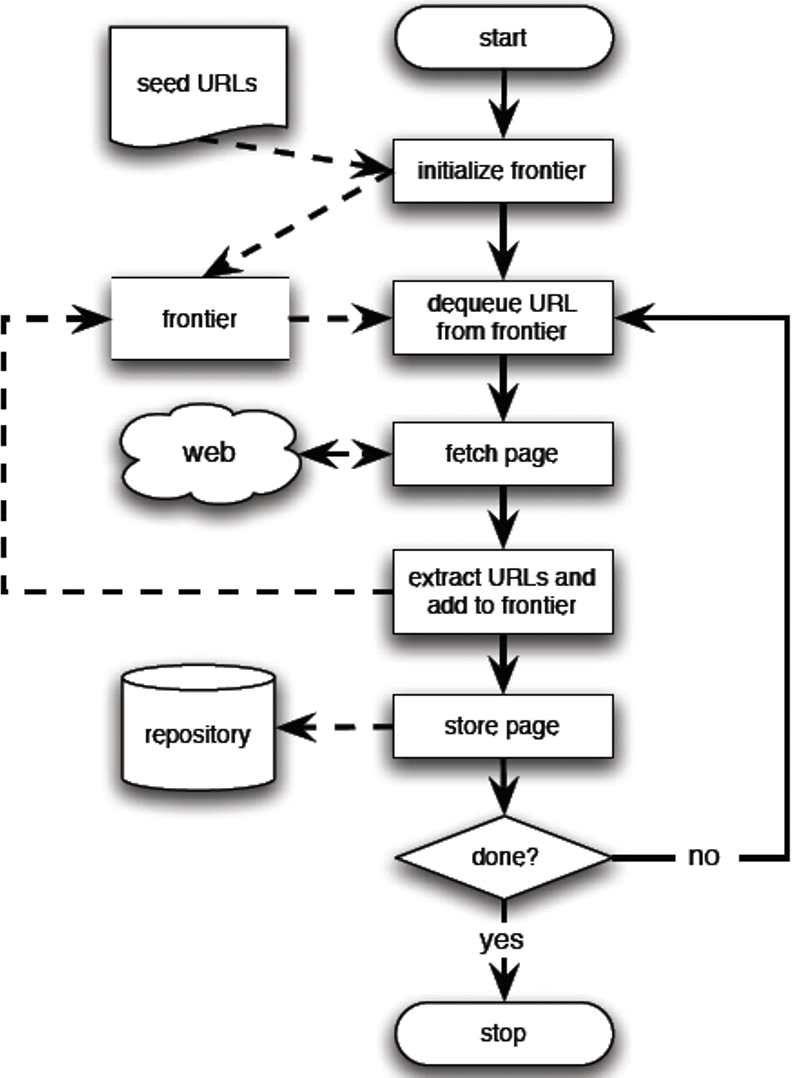
\includegraphics[width=0.5\columnwidth,keepaspectratio]{img/flowchart_webcrawler.png}
	\caption{Ablauf eines Webcrawlers}
	\source{\cite[p.313]{liu2007web}}
	\label{fig:flowchart_webcrawler}
\end{figure}
\subsection{Evaluation}
Es fand keine Evaluation zur Findung eines geeigneten Webcrawlers statt.
StormCrawler SDK wird eingesetzt, da an der Hochschule für Technik und Wirtschaft Chur ein Team bereits mit diesem arbeitet und dadurch Know-how besitzt.
Dieses Team, speziell ein wissenschaftlicher Mitarbeiter, hat Support angeboten, weshalb die Entscheidung getroffen wurde, StormCrawler SDK zu verwenden.
\subsection{Beschreibung der Technologie und Anpassungen}
Nachfolgend werden die verschiedenen Technologien beschrieben, welche verwendet wurden, um den Webcrawler zu realisieren.
\subsubsection{Apache Storm}
StormCrawler basiert auf Apache Storm, einem Opensource Framework zur verteilten Stream-Verarbeitung.
Die Architektur von Apache Storm basiert auf den folgenden Komponenten:
\begin{itemize}
	\item Spout - Komponente zum Einlesen von Daten-Streams
	\item Bolt - Komponente zum Verarbeiten von Daten-Streams
	\item Tupel - Datensatz, welcher zwischen den Komponenten weitergegeben wird
	\item Topologie - Ein Netz bestehend aus Spouts und Bolts
\end{itemize}
Jede Komponente ist als eigene Java-Klasse definiert und beinhaltet zwingend die folgenden Methoden \footnote{\url{https://dev.to/usamaashraf/playing-with-apache-storm-on-docker---like-a-boss-4bgb}}:
\begin{itemize}
	\item declareOutputFields() - Definition des Ausgabeschemas des Tupels
\end{itemize}
Jeder Bolt enthält zudem eine weitere Methode:
\begin{itemize}
	\item execute() - Ausführen des Tasks der Komponente
\end{itemize}
In einer Topologie werden verschiedene Spouts und Bolts miteinander verknüpft, um einen Prozess durchzuführen, wie in \cref{fig:topology} gezeigt wird.
\begin{figure}[H]	
	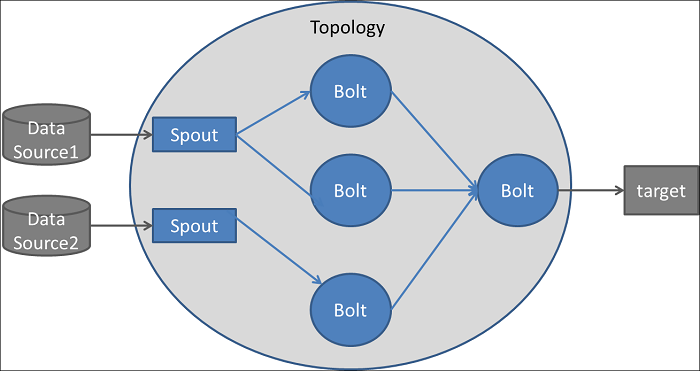
\includegraphics[width=0.8\columnwidth,keepaspectratio]{img/storm-topology.png}
	\caption{Beispieltopologie}
	\source{https://dzone.com/articles/apache-storm-architecture}
	\label{fig:topology}
\end{figure}
Dabei hat der Spout die Aufgabe, Daten aus einer Quelle (z.B. Datei, Datenbank, Array) einzulesen und daraus ein Tupel zu bilden.
Dieses Tupel wird an Bolts der Topologie weitergegeben und von diesen verarbeitet.
Diese Verarbeitung muss nicht seriell stattfinden, die Topologie kann auch Gabelungen beinhalten, die dementsprechend Bolts benötigen, welche entscheiden, an welchen Folge-Bolt das Tupel weitergegeben werden soll.
Zudem ist eine Webapplikation verfügbar, die eine Übersicht über die Informationen wie eine Topologieübersicht, der Status der jeweiligen Komponenten sowie Fehlermeldungen anzeigt.
\subsubsection{StormCrawler SDK}
StormCrawler SDK ist ein Opensource Software Development Kit, welches auf Apache Storm aufbaut und in Java entwickelt wurde.
Er dient somit als Baukasten, um einen Webcrawler aufzubauen.
Er beinhaltet verschiedene Spouts und Bolts, die explizit zum Crawlen von Websites vorgefertigt wurden\footnote{\url{https://github.com/DigitalPebble/storm-crawler/wiki}}.
Zudem berücksichtigt er die Regeln des Webcrawlings, also Meta-Tags oder Robot.txt Dateien, welche deklarieren, ob eine Website gecrawlt werden darf.
Weiter ist er so eingerichtet, dass Webpages derselben Website mit einer Zeitverzögerung abfragt, damit diese nicht überlastet werden\footnote{\url{http://stormcrawler.net/faq/}}.
StromCrawler SDK ist standardmässig so eingerichtet, dass nur Webpages desselben Hosts gecrawlt werden.
\subsection{Konfiguration des StormCrawlers}
Die Grundlage der Konfiguration ist die Standardtopologie des Stromcrawlers auf Github.
\footnote{\url{https://docs.docker.com/develop/develop-images/dockerfile_best-practices/} abgerufen am: 12.01.2019}
Diese besteht aus den folgenden Komponenten und geht wie folgt vor:
\begin{enumerate}
	\item MemorySpout - Einlesen einer URL aus einem Array
	\item URLPartitionerBolt - Geneneriert einen eindeutigen Partition Key
	\item FetcherBolt - Ruft die Webpage ab
	\item SiteMapParserBolt - Erkennt die Sitemap-Datei und fügt weitere URLs zum MemorySpout hinzu
	\item FeedParserBolt - Extrahiert URLs aus Feeds
	\item JSoupParserBolt - Extrahiert Informationen wie Metatags oder den Text aus der Webpage
	\item SdtOutIndexer - Gibt die Informationen einer Webpage über die Konsole aus
\end{enumerate}
Ein selbst erstellter Bolt, welcher für das Schreiben des Outputs zuständig ist hat in dieser Konfiguration den StdOutIndexer ersetzt.
Dieser schreibt für jede Webpage, die erreichbar ist und gecrawlt werden darf, eine JSON Datei mit den folgenden Informationen:
\begin{itemize}
	\item \glqq date\grqq{} - Zeitpunkt, zu welchem die Webpage aufgerufen wurde
	\item \glqq text\grqq{} - Vom Webcrawler extrahierter Text, welcher die Webpage beinhaltet
	\item \glqq encoding\grqq{} - Das von der Webpage verwendete Encoding
	\item \glqq title grqq{} - Inhalt des gleichnamigen HTML-Metatags
	\item \glqq url\grqq{} - URL der Webpage
	\item \glqq content\grqq{} - Der statische HTML-Inhalt der Webpage	
\end{itemize}
Der Dateiname dieser JSON Dateien wird aus der URL der Webpage generiert. 
Sonderzeichen, die in Dateinamen nicht erlaubt sind, werden entfernt. Falls die URL länger ist, als die erlaubte Dateinamenslänge, wird diese abgeschnitten und mit einem zufälligen vierstelligen Suffix erweitert.
Zudem kommt darin eine Spracherkennung \glqq Lingua\footnote{\url{https://github.com/pemistahl/lingua} abgerufen am: 07.05.2019}\grqq{} zum Einsatz, welche anhand des Textes einer Webpage detektiert, ob sie mehrheitlich in deutsch geschrieben wurde.
Als deutsch detektierte Webpages werden in einen separaten Output-Ordner gespeichert, damit diese nachfolgend von Hand gelabelt werden können.
Trotzdem ist es wichtig, dass alle aufgerufenen Webpages gespeichert werden, damit im Anschluss des Crawlens eine Aussage gemacht werden kann, wie viele Einträge des Seeds effektiv gecrawlt wurden.
\subsubsection{Docker}
In diesem Kontext wird Docker als die Software zum Erstellen von Linux-Containern verwendet.
Diese Container können einfach kopiert, ersetzt oder auf einem anderen System verwendet werden \footnote{\url{https://www.redhat.com/de/topics/containers/what-is-docker} abgerufen am: 12.01.2019}.\\
Der Vorteil von Containern ist, dass alle Abhängigkeiten mit der ausführbaren Software in den Container gepackt werden können und somit jede Umgebung, die den gleichen Container verwendet, auch den gleichen Softwarestand besitzt.
Docker Container werden mit einem einzigen Konfigurationsfile beschrieben.
Dieses Konfigurationsfile, das sogenannte Dockerfile, definiert alle Notwendigkeiten, um den Docker Container zu realisieren.
Im Dockerfile werden Instruktionen für das Erstellen des Images definiert.
Da Dockerfiles einfache Textdateien sind, können sie, wie jeder andere Sourcecode, mit Git, SVN oder anderen Versionsverwaltungen verwaltet werden.
Durch Dockerfiles können Docker Images erstellt werden, welche wiederum den dadurch definierten Container erstellen und starten.
Grundsätzlich kann das Docker Image mit einer Klasse im Objekt-Orientierten-Programmieren verglichen werden und der Docker Container wäre eine Instanz der entsprechenden Klasse. 
\subsubsection{Docker-Compose}
Mit Docker Containern können auch Micro-Services Architekturen realisiert werden, wodurch jeder Container einen eigenen Service darstellt.
Das manuelle Starten jedes einzelnen Containers erweist sich jedoch als ineffizient, deswegen übernimmt die Software \glqq Docker-Compose\grqq{} diese Aufgabe.
Mithilfe von Docker-Compose können mehrere Docker Container verknüpft und gleichzeitig gestartet werden.
Die Abhängigkeiten zwischen den Containern wird ebenfalls mit einem Konfigurationsfile, dem Composefile, definiert.
Wahlweise können Dateiordner vom Hostsystem in einzelne Container angehängt werden, damit die Container Daten dort abspeichern oder abrufen können.
Dies ist insofern wichtig, da sobald die Container gestoppt werden, all ihre internen Daten verloren gehen.
Die Containerinhalte existieren nur so lange, wie auch die Container existieren.
Docker-Compose erstellt für alle Container in einer Gruppierung einzigartige ID-Namen, damit alle Container innerhalb der Gruppierung miteinander kommunizieren können.
\subsection{Vorgehen}
\subsubsection{Erarbeitung des Webcrawlers}
Als erstes fand eine Einarbeitung in die Thematik von Docker statt, um StormCrawler damit zu betreiben.
Apache Storm ist ebenfalls thematisiert worden, da StormCrawler darauf basiert.
Danach folgte die Einarbeitung in StormCrawler.
Stormcrawler wurde nicht direkt installiert, sondern mittels Docker-Container aufgesetzt.
Dies aus dem Grund, dass dadurch eine Skalierung einfach möglich ist.
Zudem ist die Installation hinfällig, da auf Docker Hub\footnote{\url{https://hub.docker.com/} abgerufen am: 08.01.2019} bereits fertige Images von Apache Storm und StormCrawler vorhanden sind.
Zu Beginn war das Ziel, die Standardtopologie zu verstehen.
Sobald die Standardtopologie funktionierte, fanden Anpassungen statt, welche zur Erstellung der Rohdaten für den Gold Standard dienten.
Explizit ist die Erstellung des Bolts zu erwähnen, welcher für das Schreiben der Output-Dateien zuständig ist.
Dieser wurde zudem mit einer Sprachdetektion erweitert, welche erkennt, ob die Webpage in deutsch verfasst worden ist.\\
\subsubsection{Erarbeitung des Seeds}
Als Quelle für das Abrufen von Websites dient das Seed.
Das Ziel war es, dieses mit möglichst vielen URLs von Schweizer Restaurant-Websites zu füllen.
Dafür wurden zwei Ansätze verfolgt.
Ein Verein Schweizer Restaurants, namentlich Lunch-Check\footnote{\url{https://www.lunch-check.ch/} abgerufen am: 07.01.2019} wurde angefragt, ob sie eine Liste ihrer Mitglieder zur Verfügung stellen.
Zudem wurde der OpenStreetMap-API\footnote{\url{https://www.openstreetmap.ch/} abgerufen am: 07.01.2019} genutzt, um die darin enthaltenen Restaurant-URLs abzufragen.
Die Daten aus beiden Quellen wurden zusammengeführt und dienen nun als Seed für die Abfragen des Webcrawlers.
\subsubsection{Crawlen der Rohdaten}
Das Crawlen der Rohdaten war mit diversen Komplikationen verbunden.
Die Performance des Webcrawlers war zu Beginn nicht zufriedenstellend, es wurden lediglich ca. 30 Webpages pro Minute gespeichert.
Trotzdem wurde ein erster Rohdatensatz mit dieser Performance gecrawlt, auf dem das erste manuelle Labeling durchgeführt wurde.
Bei diesem Rohdatensatz wurden nur die als deutsch detektierten Webpages gespeichert, somit konnte die Abdeckung des Seeds nicht ausgewertet werden.
Der Crawler wurde nochmals angepasst, sodass alle Webpages gespeichert werden, dies ermöglicht eine genauere Analyse der Rohdaten.
Die Spracherkennung wurde zudem so angepasst, dass die Anzahl zu erkennender Sprachen eingeschränkt wurden und die Sprachdetektion nicht für jede Webpage neu gestartet wurde, was eine massive Performancesteigerung zur Folge hatte.
Diverse weitere Crawldurchläufe wurden gemacht und die gecrawlten Daten analysiert.
Diese Analysen haben ergeben, dass einzelne Websites aus dem Seed enorm viele Webpages beinhalten, zum Teil über 30'000.
Diese URLs dieser Websites wurden aus dem Seed entfernt, da sie keine typischen Restaurant-Webseiten repräsentieren.
Für die zweite Durchführung des manuellen Labelings wurden die Rohdaten mit dem angepassten Seed neu gecrawlt.
Bei diesen Rohdaten wurde analysiert, wieviele Einträge des Seeds gecrawlt wurden.
Von 5870 Seedeinträgen konnten 1362 Einträge nicht gecrawlt werden, das entspricht etwa 20\% der Einträge.
Um eine Aussage bezüglich der nicht gecrawlten Einträge machen zu können, ist eine Stichprobe von 100 Einträgen genommen worden und genauer untersucht worden, dabei sind folgende Erkenntnisse gewonnen worden:
\begin{itemize}
	\item 34\% der Websites sind offline
	\item 25\% der Websites verlinken zu einer neuen Website
	\item 8\% der Websites haben lange Wartezeiten
\end{itemize}
Somit können mindestens 67\% der Websites aus plausiblen Gründen nicht gecrawlt werden.
Es wurde nicht erfasst, wieviele Websites über Mechanismen wie Robots.txt-File oder Metatags zur Verhinderung von Crawlern verfügen, darum könnte diese Zahl noch höher sein.
Wenn davon ausgegangen wird, dass 33\% der Websites nicht gecrawlt wurden, obwohl sie crawlbar wären, ergibt dies hochgerechnet 450 Seedeinträge oder 7\%, die nicht gecrawlt wurden.
Dieses Ergebnis war zufriedenstellend, daher wurde dieser Rohdatensatz für die Klassifizierung verwendet.
\section{Webapplikation}
\subsection{Datenaufbereitung}
Um die gesammelten Daten des Webcrawlers für die Webapplikation verwendbar zu machen, ist eine produktive Pipeline erstellt worden.
Diese hat das Ziel, die Rohdaten zu klassifizieren und die als Menüseiten klassifizierten Webpages mit Informationen bezüglich des Standorts zu versehen.
Es ist der trainierte Machine-Learning-Algorithmus \glqq Perceptron mit binärem Bag of Words\grqq{} eingesetzt worden, um die Rohdaten des Webcrawlers zu klassifizieren.
Um die Menüseiten mit Geoinformationen zu versehen, wurden die ursprünglichen Daten von Openstreetmap und Lunch Check verwendet, dies aus dem Grund, da die Daten von OpenStreetMap bereits die Koordinaten des Restaurants beinhalteten.
Die Daten von Lunch-Check waren nicht mit Geoinformationen versehen, jedoch mit den Adressinformationen.
Diese wurden genutzt, um  die Daten mittels Geocoding, genauer mit einer lokalen Installation von Nominatim\footnote{\url{https://nominatim.openstreetmap.org/}abgerufen am: 02.07.2019} mit den Geoinformationen zu erweitern.
Über den Host-Anteil der URL wurden die Menüseiten den Restaurants zugeordnet.
Somit ist aus mehreren Quellen eine einheitliche Datenstruktur im JSON-Format erstellt worden.
Diese Struktur wird in \cref{fig:json_struktur} verdeutlicht:
\begin{figure}[H]	
	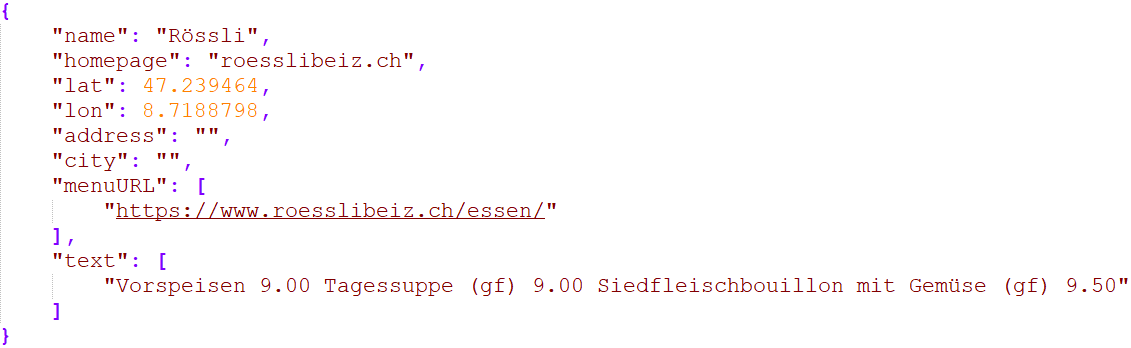
\includegraphics[width=1\columnwidth,keepaspectratio]{img/json_struktur.png}
	\caption{JSON-Struktur anhand eines Beispiels}
	\label{fig:json_struktur}
\end{figure}
\subsection{Idee}
Ziel der Webapplikation ist es, dass ein Benutzer einfach und überschaubar nach Menüs suchen kann.
Um dies zu erreichen, wurde ein Mockup mit dem Layout der Benutzeroberfläche erstellt, welches in \cref{fig:webapp_mockup} dargestellt wird.
\begin{figure}[H]
	\centering
	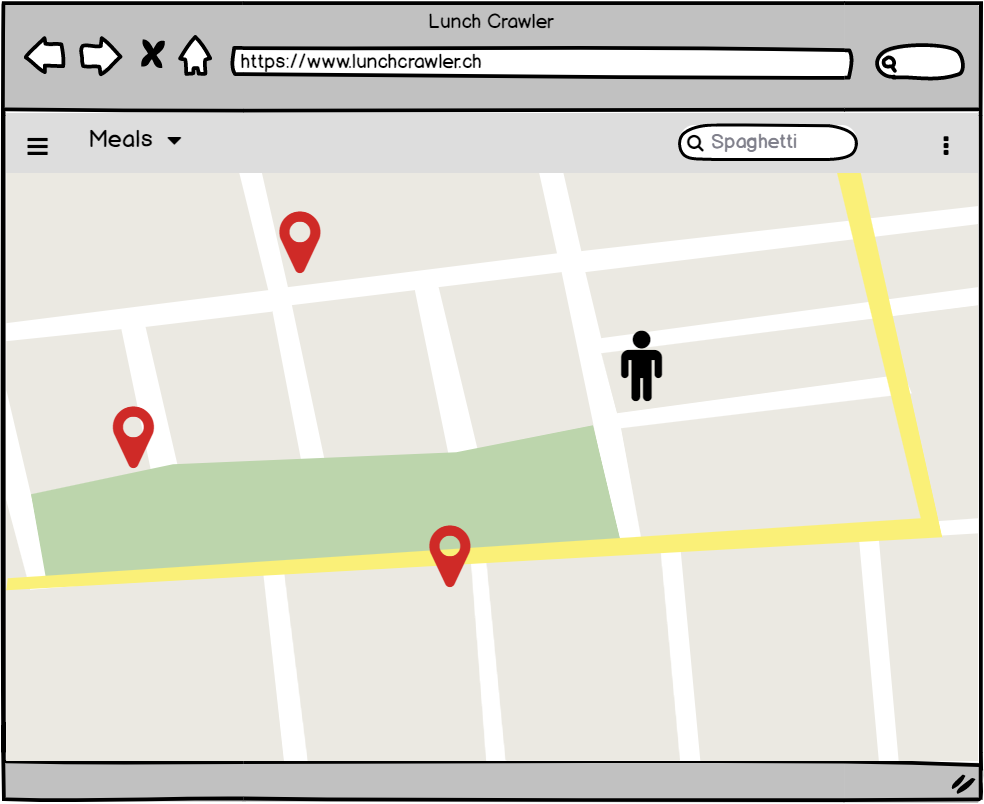
\includegraphics[width=0.7\columnwidth,keepaspectratio]{img/webapp_mockup.png}
	\caption{Mockup der Webapplikation}
	\label{fig:webapp_mockup}
\end{figure}
Dieses enthält lediglich eine Kartenansicht und einen Suchbalken.
Der Standort des Benutzers soll beim Aufruf der Webapplikation abgefragt werden, damit der Kartenfokus auf diesen gesetzt werden kann.
Durch die Eingabe einer Speise im Suchbalken werden alle Restaurants angezeigt, welche diese Speise in ihrer Menükarte führen.
\subsection{Frontend}
Das Frontend ist nach dem Prinzip einer Single-Page-Applikation aufgebaut.
Eine HTML-Datei dient als Grundgerüst und wird durch die entsprechenden JavaScript-Dateien angepasst.
Um ein ansprechendes Layout und Responsive Design zu gewährleisten, wird die Bibliothek \glqq Bootstrap\footnote{\url{https://getbootstrap.com/}}\grqq{} verwendet.
Durch die Geolocation API\footnote{\url{https://www.w3schools.com/html/html5_geolocation.asp}} wird der Standort des Benutzers abgefragt.
Das Verwenden des Suchbalkens löst eine Fetch-Anfrage auf das Backend aus.
Die Ergebnisse dieser Anfrage werden dann mit der Bibliothek \glqq Leaflet\footnote{\url{https://leafletjs.com/}}\grqq{} angezeigt.
Für jedes Restaurant wird ein Marker mit einem Popup-Fenster erstellt, welches einen Link zur Homepage sowie der Menüseite beinhaltet.
\subsection{Backend}
Als serverseitige Plattform wird \glqq Node.js\footnote{\url{https://nodejs.org/}}\grqq{} verwendet, da bereits Erfahrung mit dieser Technologie gemacht wurde und sie geeignet ist für Anwendungen dieser Grösse.
Ein Aufruf der Basis-URL stellt die HTML-Datei sowie die entsprechenden JavaScript-Dateien des Frontends zur Verfügung\footnote{\url{https://github.com/s-santoro/lunch-crawler/blob/master/webapp-lunch-crawler/routes/index.js}}.
Das Verwenden des Suchbalkens gibt die Informationen über den Standort sowie das Such-Query an das Backend weiter.
Dieses löst eine Fetch-Anfrage auf Elasticsearch aus, welche die entsprechenden Resultate als JSON zurückliefert.
Diese JSON-Dateien werden dann an das Frontend weitergeleitet.
\subsection{Search Engine}
Als Search Engine wird die Software \glqq Elasticsearch\grqq{} eingesetzt\footnote{\url{https://www.elastic.co/de/products/elasticsearch}}.
Da StormCrawler SDK entsprechende Komponenten zur Anbindung anbietet\footnote{\url{http://stormcrawler.net/getting-started/}} und dies in Betracht gezogen wurde, wird diese Software eingesetzt.
Elasticsearch wird in einem Docker-Container betrieben\footnote{\url{https://www.elastic.co/guide/en/elasticsearch/reference/current/docker.html}}.
Daten können im JSON-Format mittels HTTP-Request (POST) darin abgelegt werden\footnote{\url{https://www.elastic.co/guide/en/elasticsearch/reference/current/docs-index_.html}}.
Ebenfalls mittels HTTP-Request (GET) können Suchabfragen auf die darin enthaltenen Daten getätigt werden\footnote{\url{https://www.elastic.co/guide/en/elasticsearch/reference/6.4/search-search.html}}.
Durch diese Funktionalität nimmt Elasticsearch in diesem Fall die Funktion einer Datenbank ein.
\subsection{Benutzung der Webapplikation}
